\newpage
\subsection{Access and Additional Resources}
% Just write about where and in which forms The DesignAPI is available.
To make The DesignAPI available to as many people as possible a website has been coded.
Designers and developers can flick through digital versions of all cards and can access additional
resources that help with integrating the developed cards into the day-to-day business. The website
is available at https://designapi.netlify.app. 

% NOTE DONE: Add graphics of thumbnails maybe
\begin{description}
    \item[Figma Community File: The DesignAPI - Cards] Every card available packaged into a Figma
    Community file with a detailed description of why they were created and what the cards are
    supposed to help with.
    \item[Figma Community File: The DesignAPI - Message Templates] All message templates together
    with a detailed tutorial on how to use these templates, so even inexperienced developers can use
    this Figma Community file.
    \item[Print-at-Home: DIY DesignAPI Cards] For anyone who likes having the cards in a physical
    form rather than digital, this DIY cards template has been created. Crafting the cards could
    also be a fun activity for students learning all about UI design.
    \item[Print-at-Home: Workshop Template] This workshop template gives team members or even
    teachers the chance to make an impact with the cards. A tutorial has been added for how such a
    workshop could look like, but it has been designed to encourage teams to come up with a
    fun idea of their own! 
    \item[Print-at-Home: The DesignAPI - Poster] This poster serves the purpose of being reminded
    that qualitative design-developer collaboration is important. Posters like this could positively
    affect team culture. It includes all designed cards and a QR-Code that links to the website. 
    \item[Print-at-Home: Superstar-Card Holder] Another way to bring knowledge and awareness into
    the office is the Superstar-Card Holder. It can be folded up into a rigid construction that can
    hold one card at a time. In the office, you could crown one interesting card to be the
    Superstar-Card of this day/week/month. This way, teams are slowly informed about certain topics
    that are relevant right now.
\end{description}

With the website and additional resources in place, it is ensured that everyone can find, access and
use The DesignAPI as intended. Also, cards can be added or updated easily through the website and
the Figma Community files. This way everyone using The DesignAPI is sure to be up-to-date.

\newpage
\begin{figure}[H]
    \centering
    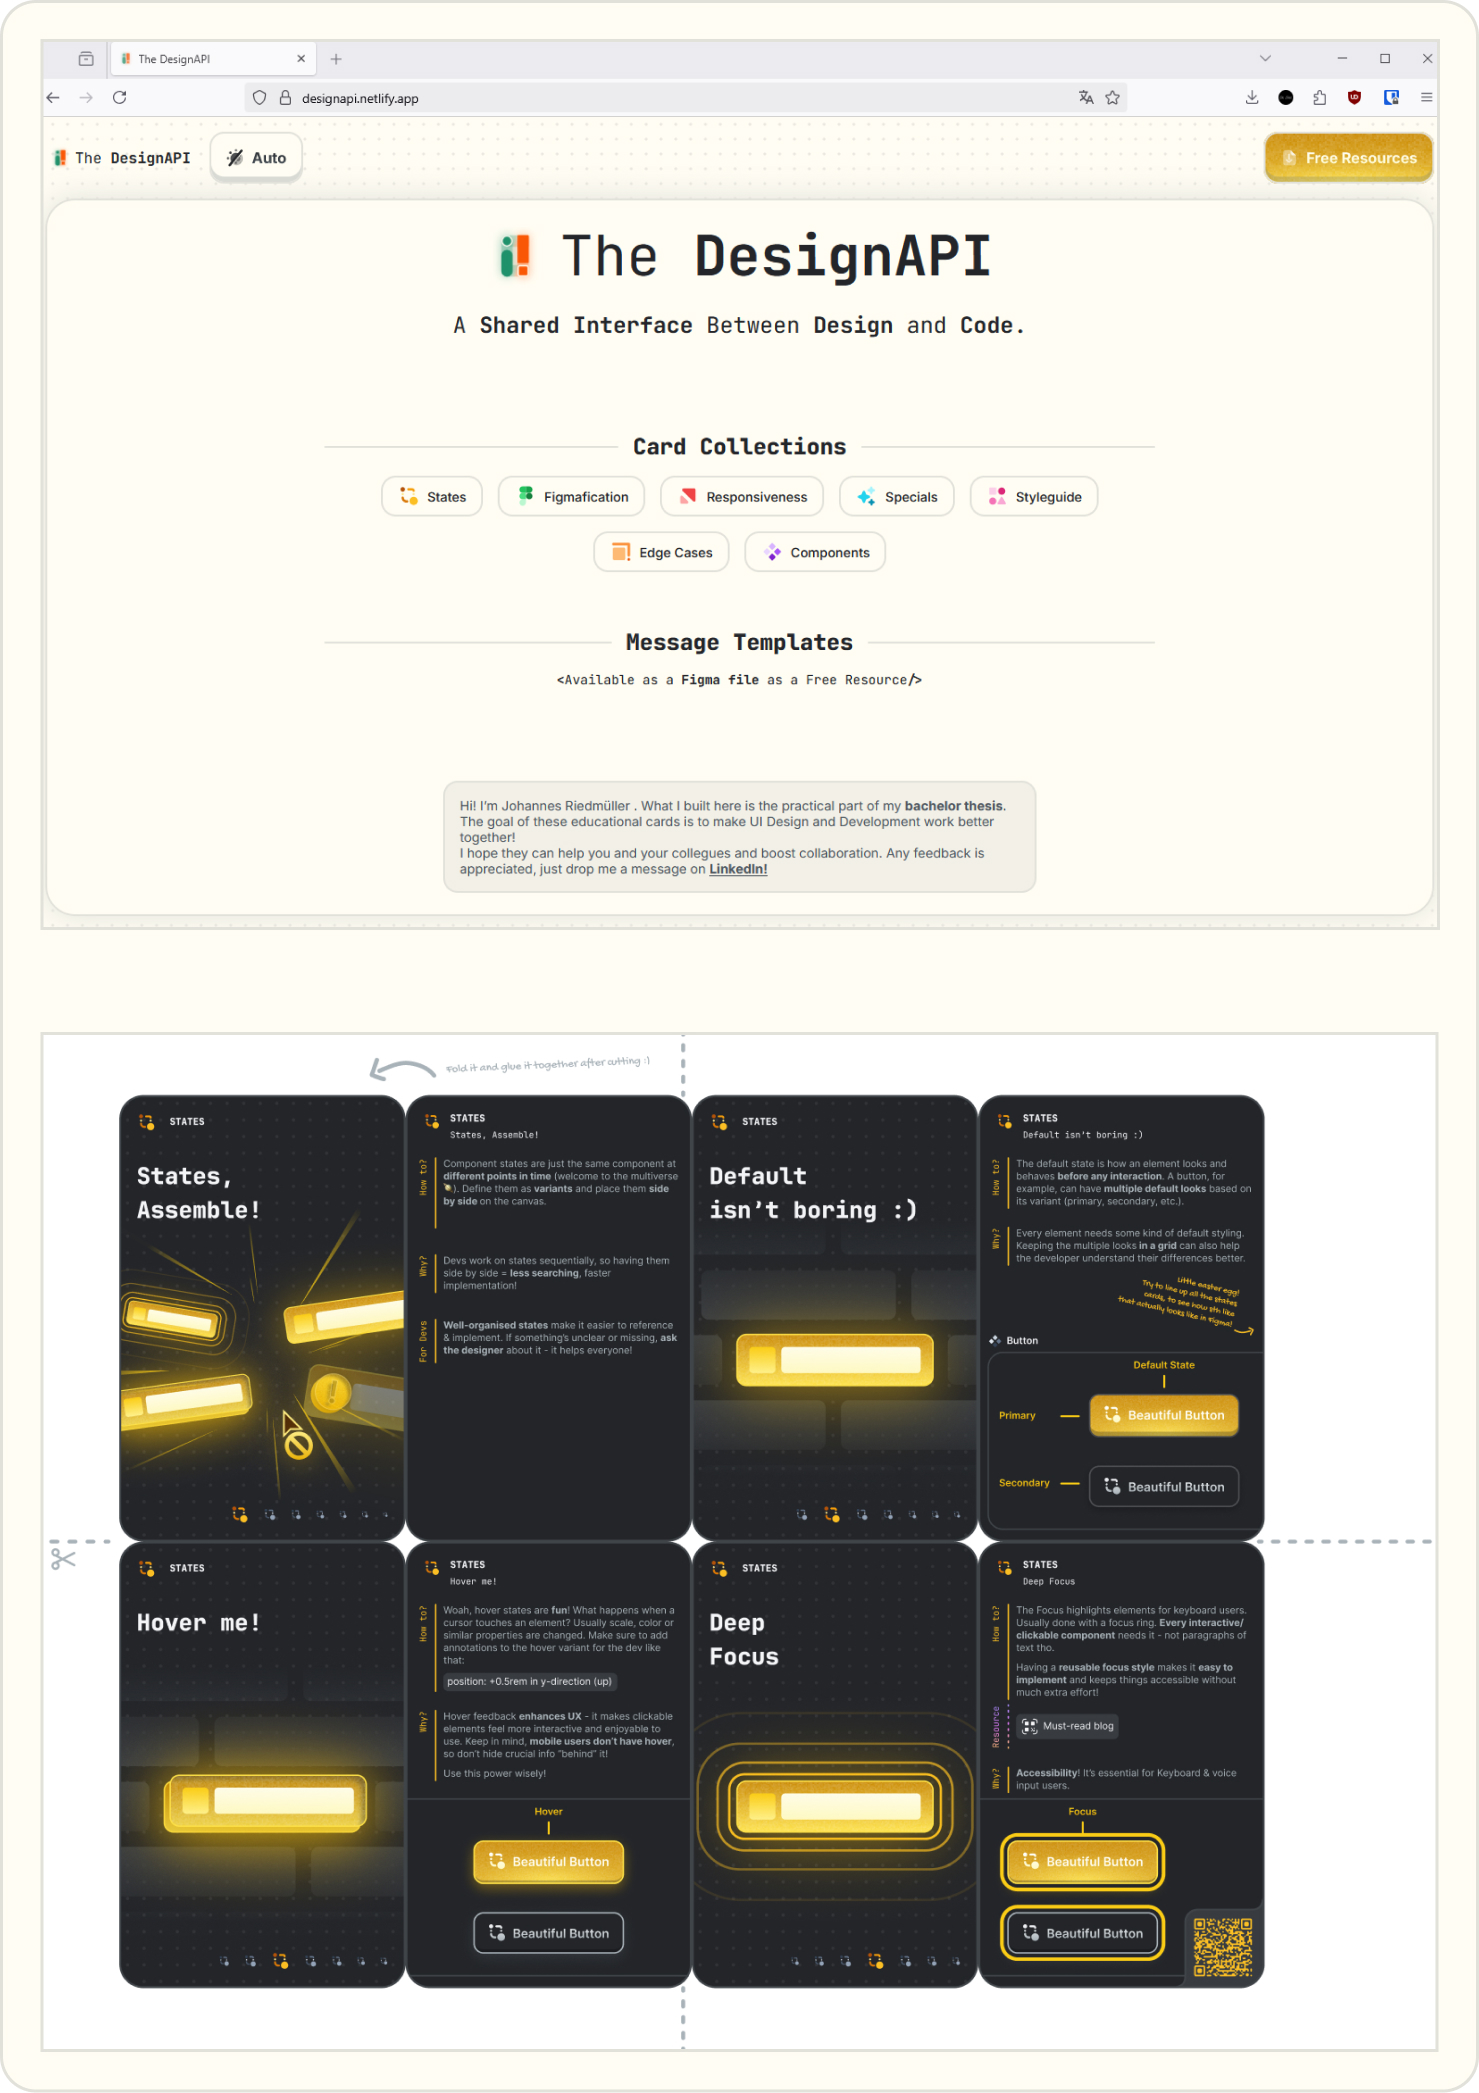
\includegraphics[width=400pt]{Chapter 6/Website and DIY Cards.jpg}
    \caption{The DesignAPI: Website and DIY cards (Source: own illustration)}
\end{figure}

\newpage
\begin{figure}[H]
    \centering
    \includegraphics[width=400pt]{Chapter 6/Superstar Card Front and Back-1.jpg}
    \caption{The DesignAPI: Workshop template and poster (Source: own illustration)}
\end{figure}

\newpage
\begin{figure}[H]
    \centering
    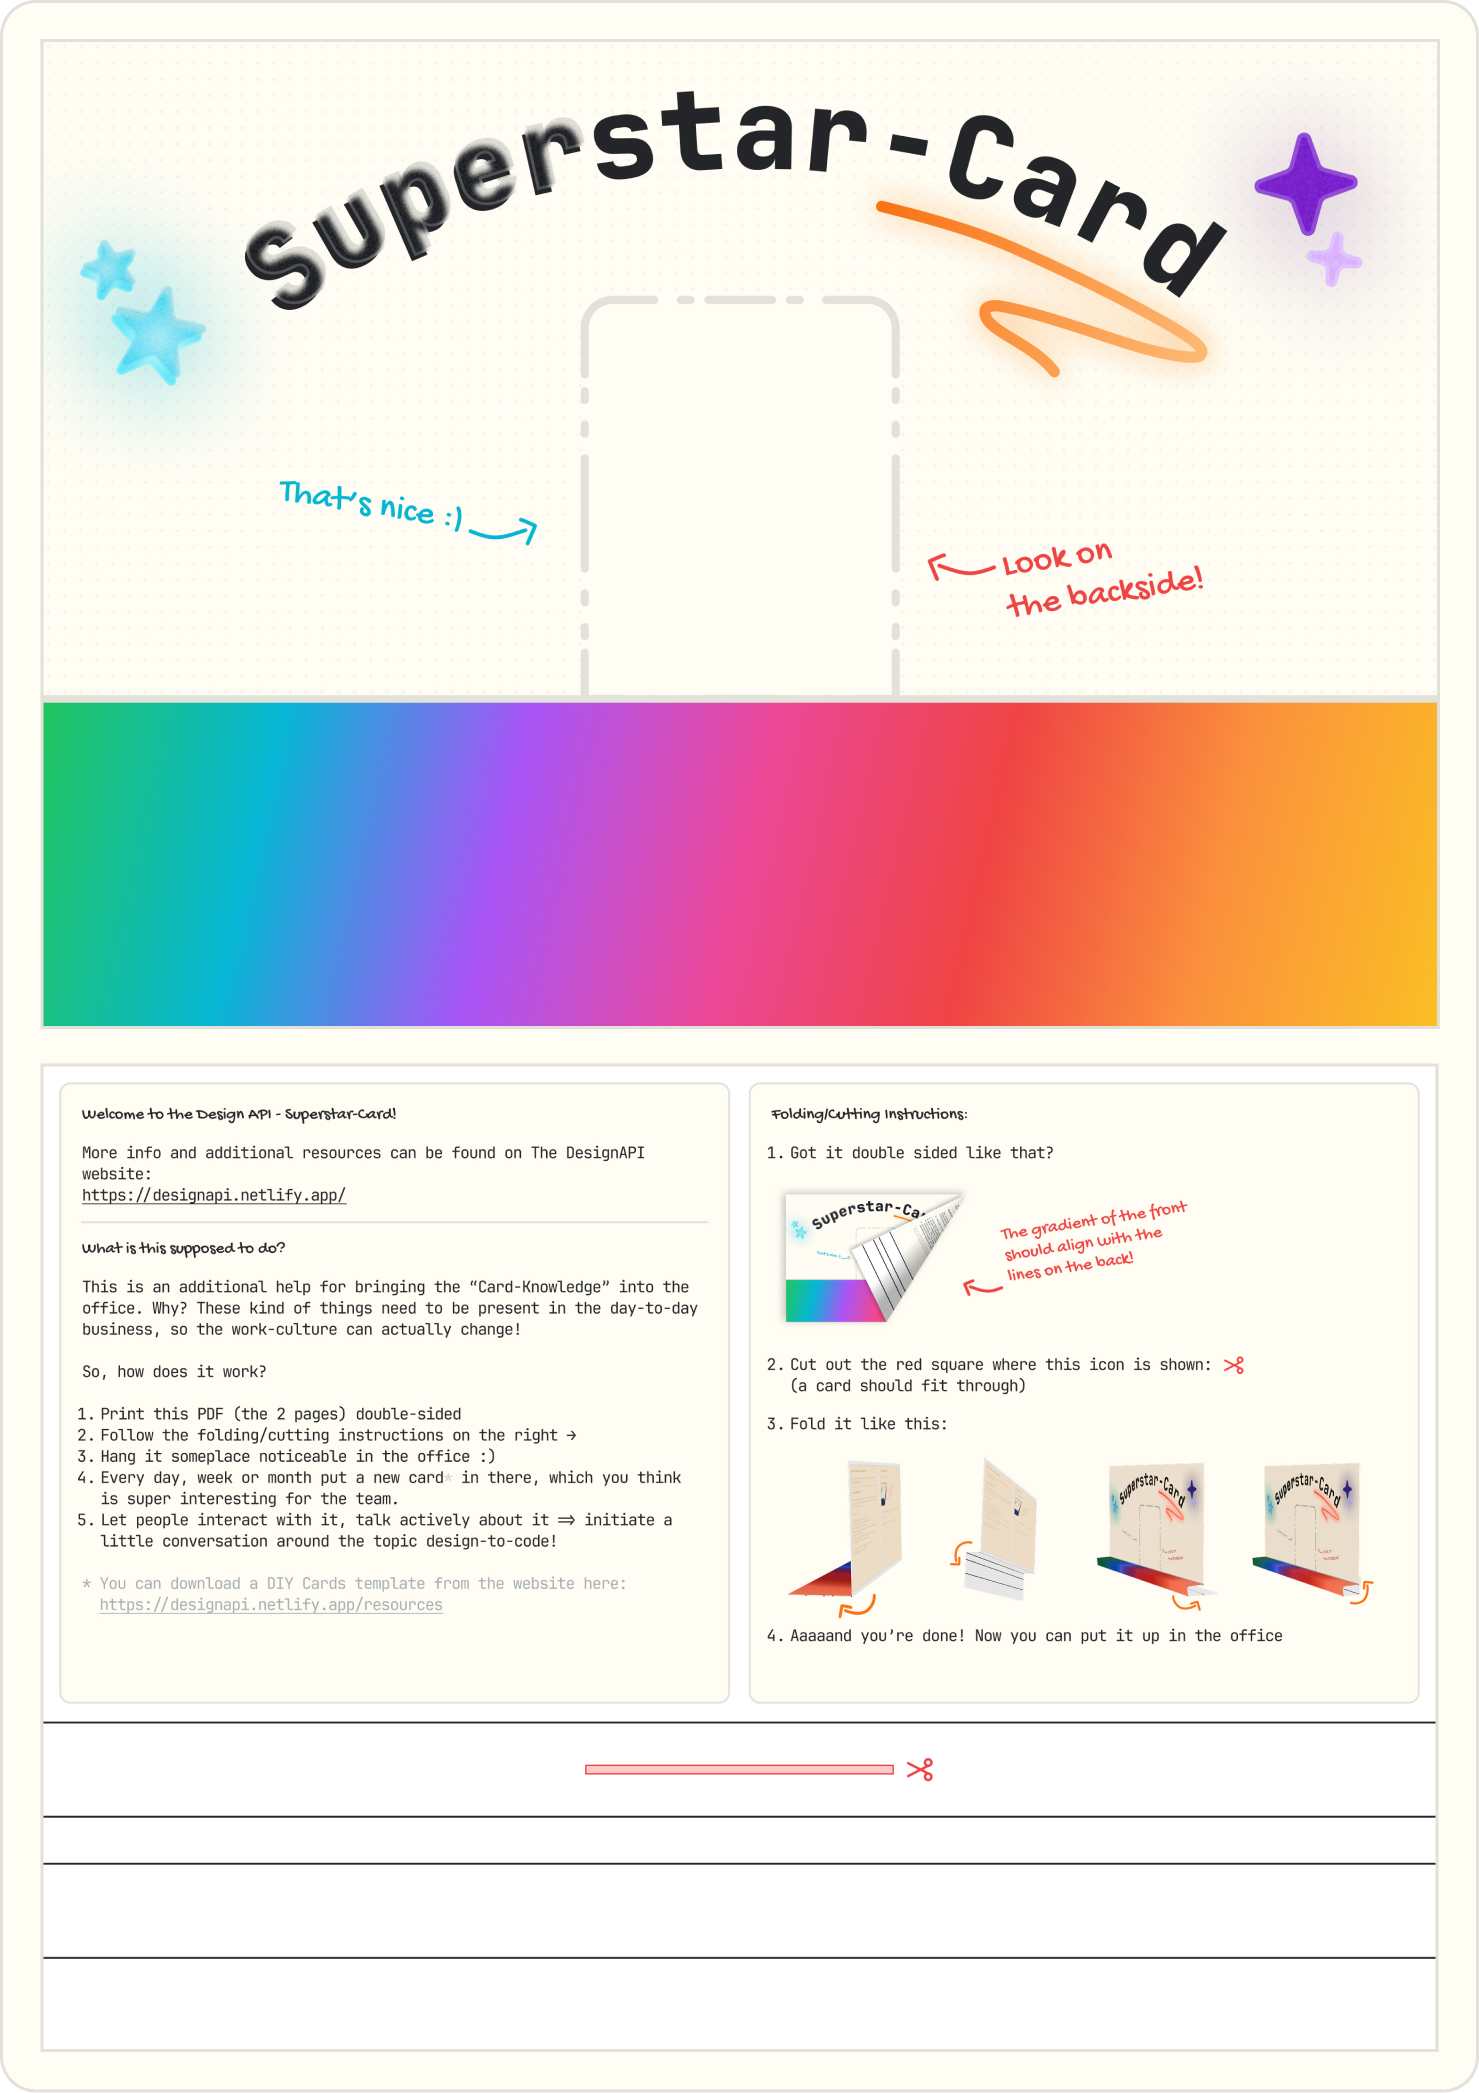
\includegraphics[width=400pt]{Chapter 6/Superstar Card Front and Back.jpg}
    \caption{The DesignAPI: Superstar-Card holder front and back (Source: own illustration)}
\end{figure}